\documentclass[tikz,border=5pt]{standalone}
\usetikzlibrary{
    matrix,
    positioning
}

\def\hsep{3em}
\def\vsep{8em}
\tikzset{
    base/.style={
        draw,
        minimum height = 1cm,
        minimum width  = 2cm,
        inner ysep=2pt,
    },
    box/.style = {
        matrix of nodes,
        row sep = 2pt,
        nodes = base
    },
    comment/.style = {
        draw=white,
        minimum height = 1cm,
        minimum width  = 2cm,
    },
    comment box/.style = {
        matrix of nodes,
        nodes = comment
    },
}
\begin{document}
    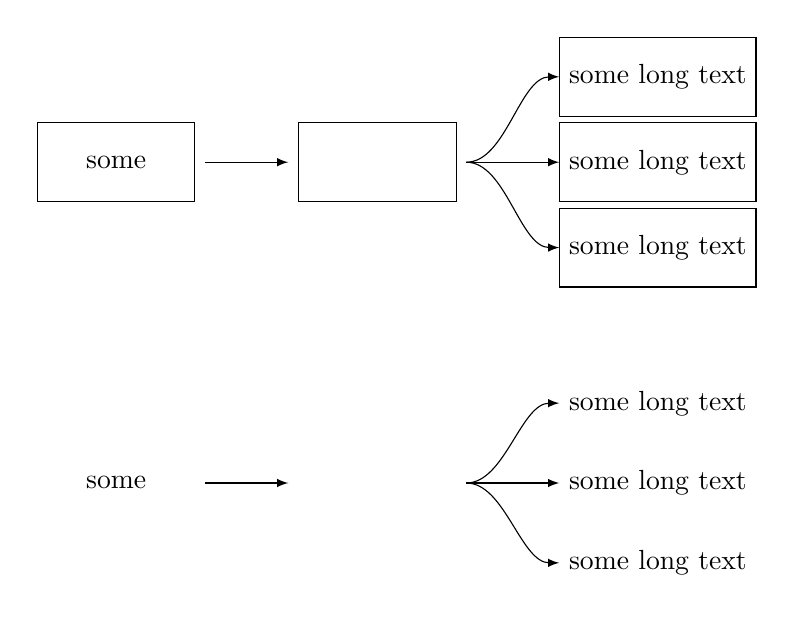
\begin{tikzpicture}
        \matrix (box1) [box] {
            some \\
        };
        \matrix (box2) [right=\hsep of box1, box] {
             ~ \\
        };
        \matrix (box3) [right=\hsep of box2, box] {
             some long text \\
             some long text \\
             some long text \\
        };

        \matrix (cbox1) [below=\vsep of box1, comment box] {
             some \\
        };
        \matrix (cbox2) [right=\hsep of cbox1, comment box] {
             ~ \\
        };
        \matrix (cbox3) [right=\hsep of cbox2, comment box] {
             some long text \\
             some long text \\
             some long text \\
        };

        \draw [-latex](box1.east) to (box2.west);
        \draw [-latex](cbox1.east) to (cbox2.west);
        \foreach \i in {1,2,3}{
            \draw [-latex, looseness=0.8, out=0, in=180](box2.east) to (box3-\i-1.west);
            \draw [-latex, looseness=0.8, out=0, in=180](cbox2.east) to (cbox3-\i-1.west);
        }

    \end{tikzpicture}
\end{document}
